%%%%%%%%%%%%%%%%%%%%%%%%%%%%%%%%%%%%%%%%%%%%%%%%%%%%%%%%%%%%%%%%%%%%%%%%%%%
%% This file is part of the book
%%
%% Algorithmic Graph Theory
%% http://code.google.com/p/graph-theory-algorithms-book/
%%
%% Copyright (C) 2009, 2010, 2011 Minh Van Nguyen <nguyenminh2@gmail.com>
%%
%% See the file COPYING for copying conditions.
%%%%%%%%%%%%%%%%%%%%%%%%%%%%%%%%%%%%%%%%%%%%%%%%%%%%%%%%%%%%%%%%%%%%%%%%%%%

\documentclass{article}

\usepackage{subfigure}
\usepackage{tikz}
\usetikzlibrary{external}
\tikzexternalize{sample-binary-heaps-array}

\begin{document}

\begin{figure}
\subfigure[]{
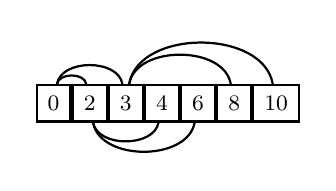
\begin{tikzpicture}
[every node/.style={inner sep=4pt,draw,thick},%
  lineDecorate/.style={-,thick}]
\footnotesize
\pgfmatrix{rectangle}{center}{}
{\pgfusepath{}}{\pgfpointorigin}{\let\&=\pgfmatrixnextcell}
{
  \node(0){$0$}; \& \node(2){$2$}; \& \node(3){$3$}; \& \node(4){$4$}; \&
  \node(6){$6$}; \& \node(8){$8$}; \& \node(10){$10$}; \\
}
\path
\foreach \startNode/\endNode/\bend in {
  0/2/bend left, 0/3/bend left, 2/4/bend right, 2/6/bend right,
  3/8/bend left, 3/10/bend left}
{
  (\startNode) edge[lineDecorate,\bend=80] (\endNode)
};
\end{tikzpicture}
}
%%
%%
\qquad
\subfigure[]{
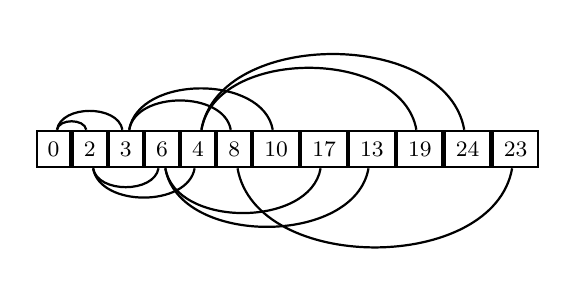
\begin{tikzpicture}
[every node/.style={inner sep=4pt,draw,thick},%
  lineDecorate/.style={-,thick}]
\footnotesize
\pgfmatrix{rectangle}{center}{}
{\pgfusepath{}}{\pgfpointorigin}{\let\&=\pgfmatrixnextcell}
{
  \node(0){$0$}; \& \node(2){$2$}; \& \node(3){$3$}; \& \node(6){$6$}; \&
  \node(4){$4$}; \& \node(8){$8$}; \& \node(10){$10$}; \& \node(17){$17$}; \&
  \node(13){$13$}; \& \node(19){$19$}; \& \node(24){$24$}; \&
  \node(23){$23$}; \\
}
\path
\foreach \startNode/\endNode/\bend in {
  0/2/bend left, 0/3/bend left, 2/6/bend right, 2/4/bend right,
  3/8/bend left, 3/10/bend left, 6/17/bend right, 6/13/bend right,
  4/19/bend left, 4/24/bend left, 8/23/bend right}
{
  (\startNode) edge[lineDecorate,\bend=80] (\endNode)
};
\end{tikzpicture}
}
%%
%%
\subfigure[]{
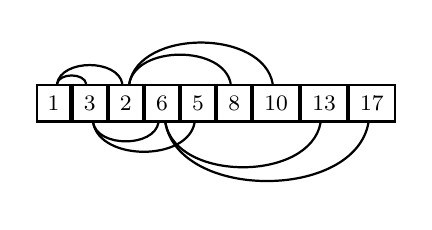
\begin{tikzpicture}
[every node/.style={inner sep=4pt,draw,thick},%
  lineDecorate/.style={-,thick}]
\footnotesize
\pgfmatrix{rectangle}{center}{}
{\pgfusepath{}}{\pgfpointorigin}{\let\&=\pgfmatrixnextcell}
{
  \node(1){$1$}; \& \node(3){$3$}; \& \node(2){$2$}; \& \node(6){$6$}; \&
  \node(5){$5$}; \& \node(8){$8$}; \& \node(10){$10$}; \&
  \node(13){$13$}; \& \node(17){$17$}; \\
}
\path
\foreach \startNode/\endNode/\bend in {
  1/3/bend left, 1/2/bend left, 3/6/bend right, 3/5/bend right,
  2/8/bend left, 2/10/bend left, 6/13/bend right, 6/17/bend right}
{
  (\startNode) edge[lineDecorate,\bend=80] (\endNode)
};
\end{tikzpicture}
}
\end{figure}

\end{document}
